\documentclass[twocolumn,10pt]{article}
\usepackage{geometry}
\usepackage{amsmath}
%\usepackage[cmintegrals]{newtxmath}
%\usepackage{bm} % optional
\usepackage{cite}
%\usepackage[dvipdfmx]{graphicx}
\usepackage{graphicx}
\usepackage{color}
\usepackage{lscape}
\usepackage{bm}
\usepackage{fancybox}
\geometry{left=20mm,right=20mm,top=10mm,bottom=10mm}
\thisfancyput(13.0cm,1.0cm){\textcolor{red}
 {\doublebox{\large{\bf{Do Not Disclose}}}}}
\begin{document}
\title{Applications of Deep Metric Learning for \\ Classification and Distillation}
\author{M181021 Hideki Oki \\ Department of Information Engineering}
\date{\empty}

\maketitle

\begin{abstract}
Metric learning is a machine learning approach based on the distance between samples.
The goal of metric learning is to learn an embedded space where the distance between similar objects is short and the distance between dissimilar objects is long.
Metric learning has various uses because of its characteristics.

With metric learning, the dataset can be converted into embedding arranged for each object.
This may provide a good embedding space for various tasks.
Therefore, we try to apply the concept of metric learning to various tasks.

First, we propose to apply metric learning to the optimization problem of ROC curves in binary classification.
We also propose an extended method for multi-class classification.
As a result, in the evaluation area under the ROC curve (AUC), we succeeded in obtaining higher performance than the conventional classifier.

Second, we propose to introduce metric learning concept  into  knowledge  distillation.
The  functionality  of  the metric  learning  to  reduce  the  differences  between  similar outputs  can  be  used  for  the  knowledge  distillation  to  reduce the differences between the outputs of deep or ensemble models (teacher model) and a smaller shallow model (student model). 
Also, since  the  outputs  of  the  teacher  model for  different  objects  are  usually  different,  the  student  model needs  to  distinguish  them.  
We  think  that  metric  learning  can clarify  the  difference  between  the  different  outputs,  and  the performance of the student model could be improved.
The effectiveness of the proposed approach is experimentally confirmed for image classification tasks.

This thesis describe these attempts.
\end{abstract}

\thispagestyle{empty}
\section{Introduction}
Metric learning is a machine learning approach based on the distance between samples.
The goal of metric learning is to learn an embedded space where the distance between similar objects is short and the distance between different objects is long.
Metric learning has various uses because of its characteristics.
Because of the characteristic that the distance between similar objects is small, it is used for abnormality detection, face verification, image search, and the like.

Meanwhile, a deep neural network model such as deep Convolutional Neural Network (CNN) has been widely used in the field of pattern recognition since deep CNN proposed by Krizhevsky et al. \cite{Krizhevsky2012} won the ILSVRC 2012 with higher recognition accuracy than the conventional methods.
Along with that, the concept of metric learning has also been introduced to deep learning.
Bromely et al. \cite{Bromely1994,Chopra2005,Hadsell2006} proposed the Siamese Neural Network as a deep metric learning model.
Siamese Neural Network is a deep learning model that performs pairwise learning.
Siamese Neural Network learns embedding to minimize the distance between similar samples and to maximize the distance between dissimilar samples.
However, since the Siamese Neural Network was a pair-wise learning model, it was necessary to uniquely determine the concept of similarity.
To address this issue, Wang et al. \cite{Wang2014}, Hoffer et al. \cite{Hoffer2015} proposed the Triplet Network, an extension of the Siamese Network to triplet-wise.
The triplet network takes a triplet of "anchor", "positive", and "negative" as input.
The triplet network learns so that the anchor-positive distance is relatively closer than the anchor-negative distance.
Therefore, multiple similar concepts can be considered without depending on one similar concept.
Triplet Network overcomes the drawbacks of Siamese Network.

Metric learning learns embedding as a cluster for each object.
That is, the dataset can be converted into embedding arranged for each object.
This may provide a good embedding space for various tasks.
Therefore, we try to apply the concept of metric learning to various tasks.

First, we propose to apply metric learning to the optimization problem of ROC curves in binary classification \cite{Oki2019}.
We propose that the classifier learn embedding that learned similarity and dissimilarity of objects by Siamese Network.
As a result, in the evaluation area under the ROC curve (AUC), we succeeded in obtaining higher performance than the conventional classifier.
We also propose an extended method for multi-class classification.
In the case of multi-class as well, we succeeded in obtaining higher performance than conventional classifier.

Second, we propose to introduce metric learning concept  into  knowledge  distillation \cite{Oki2020}.
Knowledge distillation is a technique for transferring knowledge of deep or ensemble models with many parameters (teacher model) to smaller shallow models (student model).
Generally, the student model is optimized so as to eliminate the difference between the output of the student model and the output of the teacher model.
The  functionality  of  the metric  learning  to  reduce  the  differences  between  similar outputs  can  be  used  for  the  knowledge  distillation  to  reduce the differences between the outputs of the teacher model and the  student  model.  
Also, since  the  outputs  of  the  teacher  model for  different  objects  are  usually  different,  the  student  model needs  to  distinguish  them.  
We  think  that  metric  learning  can clarify  the  difference  between  the  different  outputs,  and  the performance of the student model could be improved.
The effectiveness of the proposed approach is experimentally confirmed for image classification tasks.

The following sections describe these attempts.
\thispagestyle{empty}
\section{Our Works}
We tried to apply metric learning to AUC optimization in image classification \cite{Oki2019} and transfer of knowledge from teacher model to student model in knowledge distillation \cite{Oki2020}.
Each section discusses each of these in detail.
\subsection{Metric Learning for optimization of AUC}
O. Chapelle et al. \cite{Chapelle2010} show that RankSVM can be used to construct a binary classifier for optimizing the AUC.
Binary classification is realized by using RankSVM and by maximizing the margin of positive sample and negative sample. 
Since the Siamese Network for rank learning uses the same loss function with RankSVM,
the Siamese Network also can be used to construct a binary classifier for optimizing the AUC.
So, we propose to use the Siamese Network for rank learning for constructing a binary classifier \cite{Oki2019}.
Then the proposed method is extended to multi-class classification problem.


\subsubsection{Binary Classification}
\begin{figure}[ht]
\begin{center}
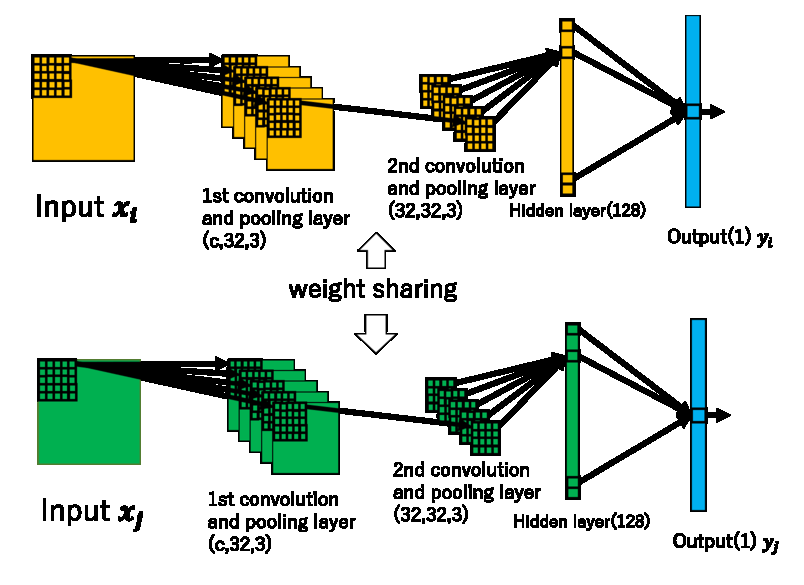
\includegraphics[width=70mm]{figure2.eps}
\caption{Siamese Network for binary classification}
\label{fig:siamese-bi}
\end{center}
\end{figure}

In order to perform binary classification, consider the Siamese Network which classify the positive class and the negative class as shown in Figure \ref{fig:siamese-bi}.
The output of each network $y$ is assumed to be scalar, namely the dimension of the output is $1$.
Similar with the standard Siamese Network, the weights of the two networks are shared.
ReLU is used as an activation function for each convolution layer and hidden layer.


The objective function of the Siamese Network for binary classification is defined as
\begin{align}
E=\frac{1}{2|\chi^2|}&\sum_{(i,j) \in \chi^2} l_{ij}(D_{ij})^2 \notag \\
&+ (1-l_{ij})max(m-D_{ij}, ~0)^2 \\
D_{ij}&=||y_{i}- y_{j}||^2_2
\label{eq:siamese-dis}
\end{align}
where $\chi^2$ is an index set of sample pairs randomly generated from the mini-batch, $m$ is a parameter indicating the distance between clusters and 
$D_{ij}$ is the distance between the pair of the outputs $y_i$ and $y_j$ of each network for the sample pair $\bm{x}_i$ and $\bm{x}_j$.
For the binary classification, the label is defined as $l_{ij}=1$ whenever the pair of inputs ${\bm x_i}$ and ${\bm x_j}$ belongs to the same class, and the label is defined as $l_{ij}=0$ whenever the pair of inputs belongs to the different class.

%Since the output is one value, $D_{ij}$ used in the contrastive loss of equation (\ref{eq:contrastive}) is changed from equation 
%(\ref{eq:dis}) as follows.
%\begin{align}
%D_{ij}&=|y_{i}- y_{j}|^2
%\label{eq:binary dis}
%\end{align}
%We assume label $t_{ij}=1$ whenever input ${\bm x_i}$ and ${\bm x_j}$ belong to the same class.
%And, we assume label $t_{ij}=0$ whenever input ${\bm x_i}$ and ${\bm x_j}$ belong to the different class.


The objective function of the Siamese Network depends on the distances between pair of samples and the order of the output of positive class $y_+$ and the output of negative class $y_-$ is not specified.
On the other hand, AUC assumes the order $y_+ > y_-$.
This means that there is a possibility to be inconsistent in the order of the outputs.
To make consistent and to estimate the posterior probability $P(l=1|\bm{x})$, we apply the logistic regression to the output of the trained network $y$. 
%At the time of model evaluation, a positive sample is input to one network and a negative sample is input to the other network, and AUC is calculated from the output result.
%And, the siamese network has no constraints on the area to cluster each class.
The logistic regression model is given by
\begin{align} \label{eq:regression}
    P(l=1|\bm{x}) \approx \hat{y} = \sigma(w y+b)
\end{align}
where $w$ and $b$ is the parameters of the model and $\sigma(\cdot)$ is the sigmoid function.
Usually the log-likelihood of the logistic regression for $N$ training samples is defined by
\begin{align} \label{eq:crossentropy}
    \hat{E} = \sum_{i=1}^N \{ t_i log(\hat{y}_i) + (1-t_i) log(1-\hat{y}_i) \} \; .
\end{align}
The optimum parameters $w$ and $b$ are obtained by maximizing this log-likelihood.

%$b$ is a bias, and $w$ is updatable weight, the gradient $\frac{\partial E}{\partial w}$ is calculated based on the loss derived from crossentropy loss(Equation (\ref{eq:crossentropy})) and it is updated by MomentumSGD.
%\begin{align} \label{eq:crossentropy}
%E = -\sum_{n}^N t_n log(\hat{y}_n) + (1-t_n) log(1-\hat{y}_n)
%\end{align}
%In the case of crossentropy loss, let the label of positive class be $t_n = 1$ and the label of negative class be $t_n = 0$.
%After 10th epoch, calculate the AUC using each $\hat{y}_n$ obtained.

In the proposed method, Siamese Network is regarded as a feature extractor and the obtained features are classified by logistic regression model.
As can be seen from Equation (\ref{eq:crossentropy}), it is obvious that the output value becomes larger for the positive class.
%Therefore, the above problem is solved. \par

%First, the average $\bar{y}$ of all output values is subtracted from each all output value $y_n$.
%\begin{align} \label{eq:avey}
 %   \acute{y}_n &= y_n - \bar{y}
%\end{align}
%As a result, the average of the output values is set to 0. \par
%Second, since there is a possibility that positive classes are clustered in the negative direction, the following %operation is performed on each output value.
%\begin{eqnarray} \label{eq:ypn}
%\hat{y}_n = \left\{
%\begin{array}{ll}
%-\acute{y}_n & (a < 0) \\
%\acute{y}_n & (otherwise)
%\end{array}
%\right.
%\end{eqnarray} 
%Here, 
%\begin{align} \label{eq:a}
%a = \frac{1}{PN}\sum_{i}^{P}\sum_{n}^{N}y_i-y_n \; .
%\end{align}
%$P$ is the total number of positive samples, and $N$ is the total number of samples.
%As a result of this operation, $\hat{y}_n$ meets the prerequisite of AUC. \par
\subsubsection{Multi-class Classification}
\begin{figure}[ht]
\begin{center}
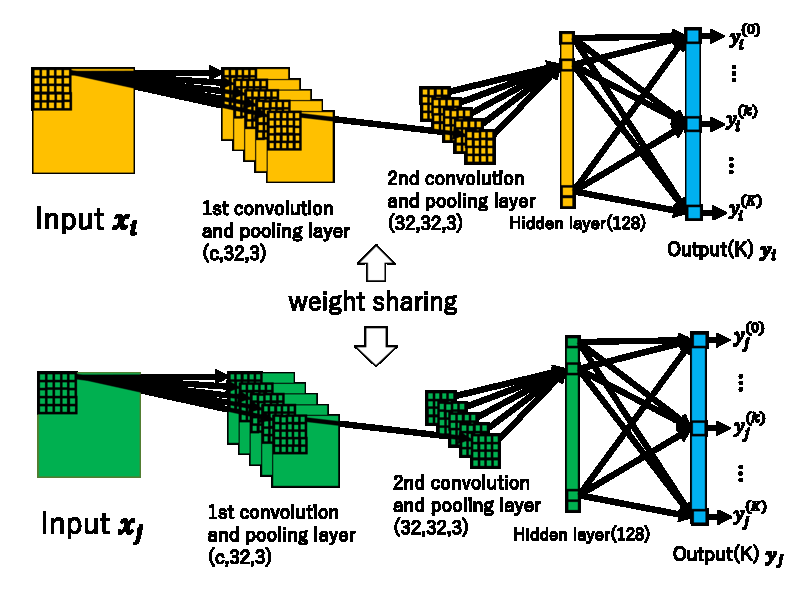
\includegraphics[width=70mm]{figure3.eps}
\caption{Siamese Network for multi-class classification}
\label{fig:siamese-mu}
\end{center}
\end{figure}
We extend the proposed binary classifier to multi-class classification by using one-vs-others approach.
%feature extractor in the binary classification proposed in the previous subsection to the multi-class feature extractor.
Figure \ref{fig:siamese-mu} shows the proposed Siamese Network for multi-class classification.
Similar with the Siamese Network for binary classification, the $K$ features $y^{(1)},y^{(2)},\ldots,y^{(K)}$ for $K$ classes classification are extracted by deep CNN.
%Each convolution layer and fully connected hidden layer are constructed in the same way as in the case of binary classification, and making the number of units of the output layer equal to the number of classes to be classified.

Each unit in the output layer of Siamese Network extracts a feature to classify the corresponding class and the other classes.
The constrastive loss of this network is defined as
%Each unit functions as a feature extractor such as in the case of a specific class and others classification. That is, considering the classification of $K$ classes now, labels are allocated to each unit, and contrastive loss is calculated for the output of each unit as shown in Equation (\ref{eq:multi contrastive}).
\begin{align} \label{eq:multi contrastive}
L_k=\frac{1}{2|\chi^2|}&\sum_{(i,j) \in \chi}^N l_{ij}^{(k)}(D^{(k)}_{ij})^2 \notag \\
&+ (1-l_{ij}^{(k)})max(m-D^{(k)}_{ij}, ~0)^2 \\
D^{(k)}_{ij}&=|y^{(k)}_{i}- y^{(k)}_{j}|^2
\end{align}
Where $\chi^2$ is an index set of sample pairs randomly generated from the mini-batch, $l^{(k)}_{ij}$ is a label in the binary classification when the $k$-th class is regarded as a positive class and the other classes are regarded as a negative class.
The distance $D^{(k)}_{ij}$ is defined as the distance between the pair of outputs $y_i^{(k)}$ and $y_j^{(k)}$ of the $k$-th unit.

The average of $K$ constrastive losses $L_k$  
\begin{align} \label{eq:ave contrastive}
E = \frac{1}{K}\sum_{k}^{K}L_k
\end{align}
is used to obtain the weights of the Siamese Network.
%Then, $k$-th unit of the output layer independently learns features for classifying the $k$-th class and others. \par

To estimate the posterior probability of each class from the features calculated by the Siamese Network, we use the multi-nominal logistic regression.
%Also in the case of multi-class classification, the problem of output described in the previous subsection occurs.
%Therefore, we extend the linear regression model described in the previous subsection for multi-class classification. \par
%In the case of multi-class classification, the number of output dimensions of siamese network is the number of classes to be classified.
The model of the multi-nominal logistic regression for the input vector $\bm{y}_n$ is given as
%So, the model of Equation (\ref{eq:regression}) is modified as follows.
\begin{align} \label{eq:regression multi}
    \hat{\bm y}_n = S(W\bm{y}_n+\bm{b})
\end{align}
where $W$ and $\bm{b}$ are the coefficient matrix and the bias vector respectively.
%Here, 
%\begin{align} \label{eq:string def}
%{\bm y}_n=\left[
%\begin{array}{c}
%y_n^{(0)} \\ 
%y_n^{(1)} \\
%\vdots \\
%y_n^{(K)}
%\end{array}
%\right], \hspace{0.2cm}
%W =\left[
%\begin{array}{ccc}
%w_{00} & \cdots & w_{0K} \\ 
%\vdots & \ddots & \vdots  \\
%w_{K0} & \cdots & w_{KK} \\
%\end{array}
%\right]
%\end{align} 
%Each element of ${\bm w}$ is an updatable weight and ${\bm b}$ is a bias. 
Also, $S(\cdot)$ is a softmax function.
%In the case of multi class, the label ${\bm t}$ expresses which class a specific sample belongs with one-hot-vector.
Similar with the binary logistic regression, the log-likelihood for the training samples is defined as
\begin{align} \label{eq:multi crossentropy}
\hat{E} = \sum_n^N {\bm t}_n^Tlog(\hat{\bm y}_n) \; 
\end{align}
where $log(\hat{\bm y}_n)$ is the logarithm of each element of $\hat{\bm y}_n$. 
This is used to obtain the optimum parameters $W$ and $\bm{b}$ of the model.
It is known that this log-likelihood is the same as the cross entropy loss except the sign.
%\par
%As in the previous subsection, the optimum parameters ${\bm w}$ and ${\bm b}$ are obtained by maximizing this log-likelihood. \par

\thispagestyle{empty}
\subsection{Metric Learning for Knowledge Distillation}
\begin{figure}[h!]
\begin{center}
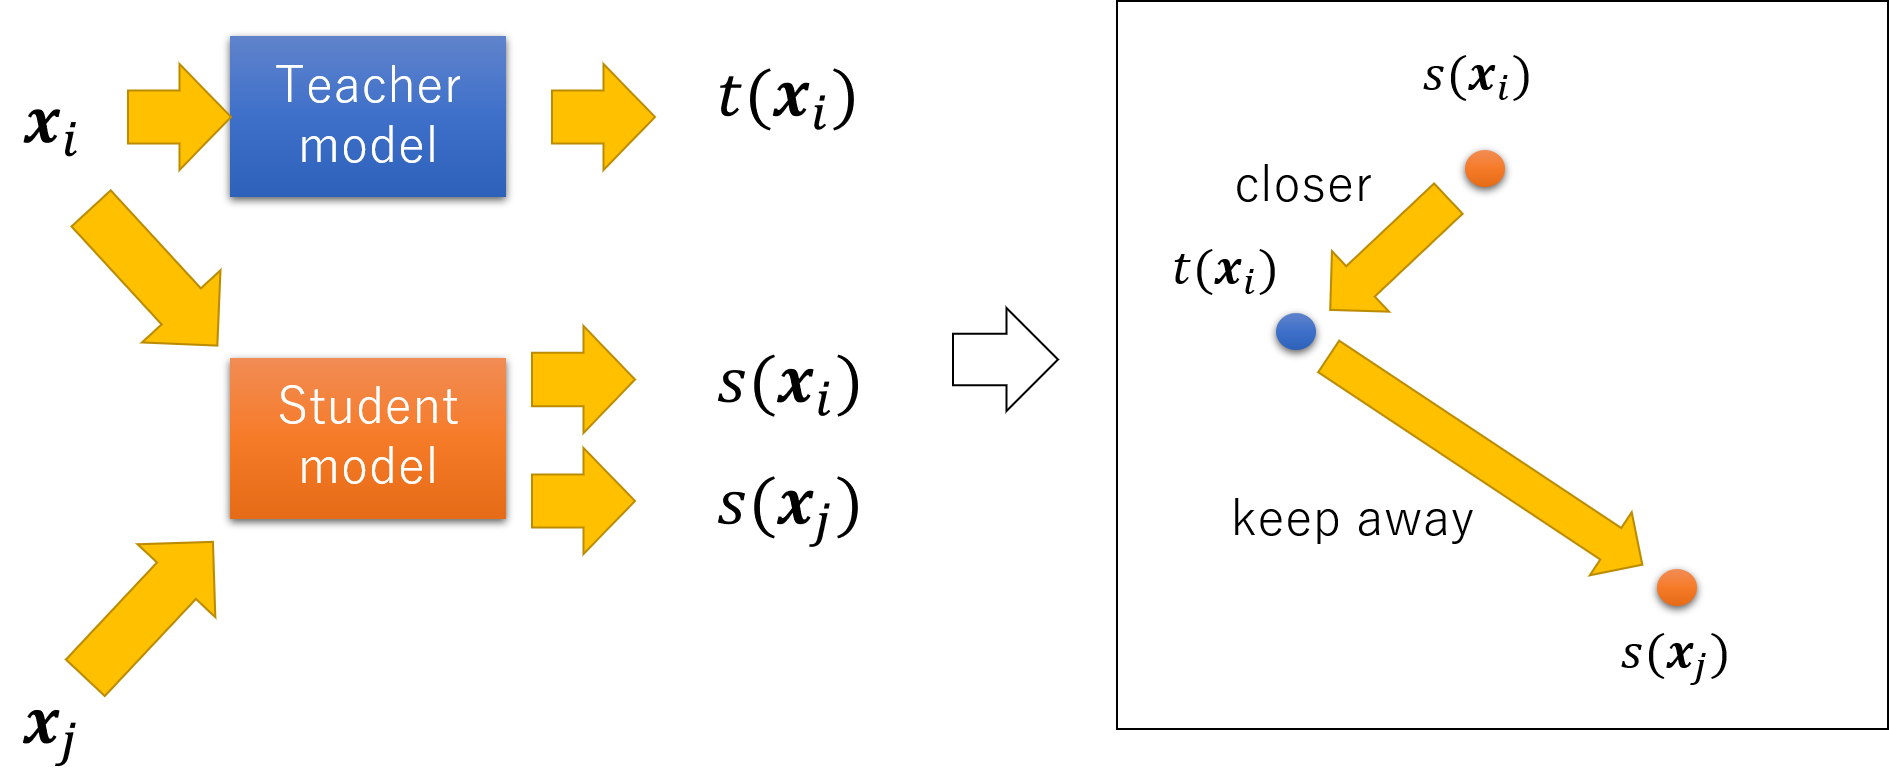
\includegraphics[width=70mm]{figure_ours.png}
\caption{The structure of our method. The student model is optimized so that its own output for sample $\bm{x}_a$ and the output of the teacher model for sample $\bm{x}_a$ are closer. At the same time, the student model is optimized so that its own output for sample $\bm{x}_n$ which is the different classes in the soft target and the output of the teacher model for sample $\bm{x}_a$ are keeping away.}
\label{fig:ours}
\end{center}
\end{figure}

Previously proposed methods of knowledge distillation focused on minimizing the difference between the teacher model and the student model in order to transfer knowledge of the teacher model.
In other words, they are solving the optimization problem in which the similarity between the function of the teacher model and the function of the student model is maximized.
There is a possibility that knowledge of the teacher model can be transferred to the student model by using the metric learning method to embed the neighboring relations of the teacher model in the output space of the student model.

Triplet \cite{Wang2014},\cite{Hoffer2015}, one of the deep metric learning methods, is a powerful method for learning similarity and dissimilarity.
Triplet loss has a function to reduce the output distance of "anchor-positive" and a function to increase the output distance of "anchor-negative".
We proposed to apply this technique for knowledge distillation \cite{Oki2020}.

We define the triplet loss for knowledge transfer as
\begin{align}
    E_{ourKD} = &\sum_{(a,n) \in \Omega} max(0, m + ||t({\bm x_a}) - s({\bm x_a})||_2^2 \notag \\ 
    &- ||t({\bm x_a}) - s({\bm x_n})||_2^2) \; ,
\end{align}
where $t(\cdot)$ is the output of the teacher model, $s(\cdot)$ is the output of the student model, and $m$ is the margin.
Further, ${\bm x_a}$ is a training sample extracted at random, and ${\bm x_n}$ is a sample classified into a different class from ${\bm x_a}$ in the case of a soft target.
$\Omega$ is the index set of each corresponding sample.
So, the output of the teacher model and the output of the student model for the same sample are considered as "anchor" and "positive", respectively.
Also we consider the output of the student model for samples of different classes in the case of soft target as "negative".
Since we are training the student model, the weight of the teacher model is not updated.
That is, $t(\cdot)$ is treated as a constant during training process.

For our loss, there is a term that makes the outputs of the teacher model and the student model closer. 
This is realized by making the square error of the outputs of the teacher model and the student model a loss.
This is similar to Ba et al. \cite{Ba2014} proposed function.
In addition, there are terms that increase the distance between outputs of different classes.
In other words, in addition to the conventional loss functions, it is possible to add a constraint that the student model makes the outputs of other classes dissimilar.
This will allow the student model to clarify differences in output between classes.
We have shown experimentally that this proposal contributed to the performance improvement of the student model.
We will also seek further performance improvements in combination with other distillation losses.

\thispagestyle{empty}
\section{Experiment}
In this section, we will experiment with the contributions of each of the efforts described in the previous section.
Each section describes the details of the experiment.
\subsection{Metric Learning for optimization of AUC}
In the experiment, we used Fashion-MNIST \cite{Xiao2017} dataset and CIFAR-10 \cite{Krizhevsky2009} dataset.
At first, the effectiveness of the proposed approach for binary classification is investigated by comparing the proposed method with the standard CNN. Then the effectiveness for multi-class classification is investigated.
\subsubsection{Binary Classification}
At first we consider binary classification problems in which a specific target class and the other classes are classified.
Since there are ten classes in the datasets (Fashion-MNIST and CIFAR-10), we trained ten different networks for binary classification.
The Siamese Networks for binary classification shown in Figure \ref{fig:siamese-bi} are trained.
Then the parameters of the logistic regression model are determined to estimate the posterior probability of the target class.

For the comparison, the standard CNN with the same network structure with the Siamese Network is also trained as the baseline model.
The sigmoid function is used as the activation function of the output layer of the standard CNN and the binary cross entropy is used as the loss function.
AUC scores for the proposed model and the standard CNN are calculated.

The average AUC scores for Fashion-MNIST dataset are shown in Table \ref{tabel:AUC_Fashion_binary}.
Table \ref{table:AUC_CIFAR10_binary} shows the average AUC scores for CIFAR-10 dataset.
It is noticed that the average AUC scores of the proposed method are better than the standard CNN for many cases.
%The results show that in the binary classification of Fasion-MNIST and CIFAR10, the feature vector of siamese network improves the ROC-AUC score in many cases.
Especially for CIFAR-10 dataset almost all the average AUC scores of the proposed method are better than the standard CNN. 


%On the other hand, the baseline model, which is the object of comparison, consists of one network that outputs one value as shown in Figure 2.
%The sigmoid function is used as the activation function of the output layer, and the AUC is calculated from the output $y$ of the network. \par
%In the comparative experiment,  10-class datatset is used, and AUC scores of each model are compared by binary classification which classifies one specific classes (target class) and other classes.


%We consider binary classification which classifies a specific target class and other samples using the dataset mentioned above.
%We compare AUC of baseline model and AUC of siamese network when each class is taken as the target class.

%In addition, for each model, experiments are conducted with five kinds of initial weight values, and this average score is posted as a result. \par
%In order to prevent over learning, regularization term is added to loss as necessary.
%The AUC score in the binary classification that classifies the target class and the other classes is shown in the following Figure \ref{fig: binary auc fasion} and \ref{fig: binary auc cifar}.
%For the class "coat" of fasion mnist dataset and the class "deer" of CIFAR10 dataset, the result of binary classification is shown by ROC curve (Figure \ref{fig:roc-bi}). \par
%It is noticed that the proposed method is better than the standard CNN classifier.

\begin{table}[ht]
\begin{center}
\caption{AUC of binary classification (Fasion-MNIST)}
\label{tabel:AUC_Fashion_binary}
\scalebox{0.65}{
\begin{tabular}{|c|c|c||c|c|c|} \hline
target class & Baseline & Siamese & target class &  Baseline & Siamese  \\ \hline \hline
class "t-shirt" &  ${\bf 0.9889}$       &     $0.9850$            &   class "sandal"        &  $0.9996$   &  ${\bf 0.9998}$   \\ \hline
class "trouser" &    $0.9992$   &         ${\bf 0.9999}$        &  class "shirt"          & ${\bf 0.9723}$   &   $0.9720$   \\ \hline
class "pullover" &    ${\bf 0.9891}$         &  $0.9854$               &  class "sneaker"          &  $0.9989$  &  ${\bf 0.9990}$    \\ \hline
class "dress" &   ${\bf 0.9955}$          &    $0.9928$            &     class "bag"      & $0.9985$       & ${\bf 0.9996}$ \\ \hline
class "coat" &   $0.9891$          &         ${\bf 0.9909}$       &    class "ankle boot"          & $0.9988$   & ${\bf0.9989}$    \\ \hline
\end{tabular}
}
\end{center}
\end{table}


\begin{table}[ht]
\begin{center}
\caption{AUC of binary classification (CIFAR-10)}
\label{table:AUC_CIFAR10_binary}
\scalebox{0.65}{
\begin{tabular}{|c|c|c||c|c|c|} \hline
class & Baseline & Siamese & class &  Baseline & Siamese  \\ \hline \hline
class "airplane" &     $0.9554$    &     ${\bf 0.9599}$          &   class "dog"        &$0.9292$     &  ${\bf 0.9323}$  \\ \hline
class "automobile" & $0.9783$      &    ${\bf 0.9827}$          &  class "frog"          & $0.9710$   &  ${\bf 0.9719}$    \\ \hline
class "bird" &     $0.9066$        & ${\bf 0.9076}$              &  class "horse"          & $0.9630$   & ${\bf 0.9653}$    \\ \hline
class "cat" &        ${\bf 0.8879}$     &    $0.8581$            &     class "ship"      &  $0.9771$      & ${\bf 0.9789}$ \\ \hline
class "deer" &     $0.9303$        &     ${\bf 0.9402}$           &    class "truck"          &  $0.9735$  & ${\bf 0.9785}$    \\ \hline
\end{tabular}
}
\end{center}
\end{table}

\subsubsection{Multi-class Classification}
Here we investigate the effectiveness of the proposed method for multi-class classification.
The proposed model is trained by using Fashion-MNIST dataset and CIFAR-10 dataset.
As the baseline model, the standard CNN with softmax function as the activation function of the output layer is also trained to minimize the cross entropy loss.
Similar with the binary classification, the average AUC scores are measured for the proposed method and the standard CNN.
%For baseline model, learning of end to end is performed by crossentropy loss of Equation (\ref{eq:multi crossentropy}) using softmax function as the activation function of $K$ output layers.
%This is a general multi-class classifier model using a neural network. \par
%Comparison experiments compare the AUC scores of these two models.
The recognition accuracies for each model are also calculated.
%$\hat{\bm t}_n$ is a $K$-dimensional one-hot-vector with $\hat{y}_n^{(k)}$ as an element satisfying the following condition.
%\begin{align} \label{eq:accuracy}
%\hat{t}_n^{(k)}=\left\{
%\begin{array}{cc}
%1 & (k = argmax(y_n^{(0)}, y_n^{(1)}, \cdots, y_n^{(K)})) \\ 
%0 & (otherwise)
%\end{array}
%\right.
%\end{align} \par
In the case of multi-class classification, %each model is evaluated with accuracy and AUC.
we regard that each unit of the output layer solves the binary classification problem classifying the target class and the other classes and the average of the AUC scores of each output unit is calculated as the AUC score for each model.

The results are shown in Table \ref{table:AUC_ACC_multi}.
It is noticed that both of the average AUC score and the recognition accuracy of the proposed method is better than the standard CNN for multi-class classification.
%As a result of comparative experiments, also in the case of multi-class, improvement of AUC score was seen.
%And, siamese network exceeds the score in accuracy evaluation.
%By the way, in general crossentropy loss which uses sigmoid function as output activation function is used for binary classification using neural network.
%This sigmoid crossentropy considers positive and negative samples independently.
%On the other hand, the siamese network learns the metric between samples.
%As can be seen the figure, siamese network has higher accuracy and AUC score for both datasets.
Particularly in classification of CIFAR10, the recognition accuracy is about 3$\%$ better than the standard CNN.
It is noticed that the proposed method gives better results than the standard CNN.

%In  addition,  for  each  model,  experiments  are conducted  with  five  kinds  of  initial  weight  values,  and  this average score is posted as a result. \par
%The accuracy and AUC for each dataset are shown in Table \ref{table:AUC_ACC_multi}.
%In  order  to  prevent  over  learning, regularization  term  is  added  to  loss  as  necessary.



\begin{table}[ht]
\begin{center}
\caption{AUC and accuracy for multi-class classification}
\label{table:AUC_ACC_multi}
\scalebox{0.7}{
\begin{tabular}{|c|c|c||c|c|c|} \hline
AUC & Baseline & Siamese & accuracy &  Baseline & Siamese  \\ \hline \hline
fasionMNIST & $0.9932$    & ${\bf 0.9941}$  &  fasionMNIST  & $90.40\%$   &  ${\bf 91.63}\%$ \\ \hline
CIFAR10  & $0.9601$      &  ${\bf 0.9635}$     &  CIFAR10   & $72.19\%$     &${\bf 75.38}\%$ \\ \hline
\end{tabular}
}
\end{center}
\end{table}

\subsection{Metric Learning for Knowledge Distillation}
We experimentally investigated the effectiveness of the proposed method with the image classification task.
CIFAR-10 and Tiny ImageNet \cite{Le2015} are used as datasets.

\subsubsection{Experiments using CIFAR-10}

\begin{table}[ht] 
\caption{model structures for CIFAR-10}
\label{table:structure}
\begin{center}
\scalebox{0.7}{
\begin{tabular}{l|l} 
\hline
student model(5 layers) & teacher model(8 layers)   \\ \hline \hline
conv1(channel:32, filter:3) & conv1(channel:32, filter:3) \\
max pooling(2*2) & batch normalization(32) \\
conv2(channel:32, filter:3) & max pooling(2*2) \\
max pooling(2*2) & conv2(channel:32, filter:3) \\
conv3(channel:64, filter:3) & batch normalization(32) \\
max pooling(2*2) & max pooling(2*2) \\
fully-connected(128) & conv3(channel:64, filter:3) \\
output(10) & batch normalization(64) \\
 & conv4(channel:64, filter:3) \\
 & batch normalization(64) \\
 & conv5(channel:128, filter:3) \\
 &  batch normalization(128) \\
 & max pooling(2*2) \\
 & fully-connected(512) \\
 & dropout \\
 & fully-connected(128) \\
 & dropout \\
 & output(10) \\
\hline
\end{tabular}
}
\end{center}
\end{table}

In the case of CIFAR-10, the 8-layers CNN model shown in Table \ref{table:structure} was used as a teacher model, and the 5-layers CNN model was used as a student model.

An activation function ReLU is used for the outputs of each convolution layer and the outputs of each fully-connected layer except for the last output layer.

In the training, the optimization is done by using the stochastic gradient descent (SGD) with momentum.
We also introduced weight decay to prevent over-learning.


\begin{table}[ht]
\caption{Classification accuracy for CIFAR-10}
\label{table:cifar-10}
\begin{center}
\scalebox{0.8}{
\begin{tabular}{|l|l|}
\hline
method & accuracy \\ \hline \hline
Student model & $74.66\%$ \\ \hline
Ba's KD \cite{Ba2014} & $80.40\%$ \\ \hline
Hinton's KD \cite{Hinton2015} & $79.16\%$ \\ \hline
RKD-DA \cite{Park2019} &       $79.21\%$     \\ \hline
Ours KD \cite{Oki2020} & $\bm{81.14}\%$ \\ \hline \hline
Teacher model  & $83.42\%$     \\
\hline
\end{tabular}
}
\end{center}
\end{table}

The Table \ref{table:cifar-10} shows the classification accuracy of the student model for test samples in each method.
From the table, it can be seen that in the case of CIFAR10, the proposed method achieves higher performance than the other methods.

\thispagestyle{empty}
\subsubsection{Experiments using Tiny ImageNet}

Also, we have performed experiments using the Tiny ImageNet dataset.
For the case of Tiny ImageNet, VGG19 with batch normalization \cite{Simonyan2014, Ioffe2015} and VGG11 \cite{Simonyan2014} were used as the teacher model and the student model, respectively.

The weights in the convolution layers were pre-trained by using ImageNet, and they were used as the initial weights of the training.
Similarly, the SGD with momentum was used for the optimization.
We also used mixup \cite{Zhang2017} to prevent over-learning.


\begin{table}[ht]
\caption{Classification accuracy for Tiny ImageNet}
\label{table:imagenet}
\begin{center}
\scalebox{0.8}{
\begin{tabular}{|l|c|}
\hline
method & accuracy \\ \hline \hline
Student model & $58.63\%$ \\ \hline
Ba's KD \cite{Ba2014} & $59.80\%$ \\ \hline
Hinton's KD \cite{Hinton2015} & $59.80\%$ \\ \hline
RKD-DA \cite{Park2019} & $59.73\%$     \\ \hline
Ours KD \cite{Oki2020} & $\bm{60.00}\%$ \\ \hline \hline
Teacher model  & $63.17\%$    \\
\hline
\end{tabular}
}
\end{center}
\end{table}

Table \ref{table:imagenet} shows the classification accuracy of the student model for the Tiny ImageNet dataset in each method.
The results show that the proposed method gives slightly better performance than the other methods.


\subsubsection{Experiments on the combined loss}

Park et al. \cite{Park2019} succeeded in achieving even higher performance by combining their method (RKD-DA) with Hinton's method \cite{Hinton2015}.
Here we investigate the effectiveness of the combination of different loss functions.
Depending on the datasets CIFAR-10 and Tiny ImageNet, the same network architectures with the previous subsections were used.
The student models were trained, and the classification performances of the trained student models are calculated.

\begin{table}[ht]
\caption{Classification accuracy for combined with HKD}
\label{table:combined}
\begin{center}
\scalebox{0.8}{
\begin{tabular}{|l|c|c|}
\hline
method & CIFAR10 & Tiny ImageNet \\ \hline \hline
Student model &$74.66\%$  & $58.63\%$ \\ \hline
Hinton's KD \cite{Hinton2015} & $79.16\%$ & $59.80\%$  \\ \hline
Ba's KD + HKD & $80.33\%$ & $60.19\%$  \\ \hline
RKD-DA + HKD &  $79.65\%$   & $59.89\%$      \\ \hline
Ours KD + HKD & $\bm{80.93}\%$ & $\bm{60.62}\%$  \\ \hline \hline
Teacher model  & $83.42\%$  & $63.17\%$  \\
\hline
\end{tabular}
}
\end{center}
\end{table}

Table \ref{table:combined} shows the classification performance of the test samples for each dataset.
From this table \ref{table:combined}, it is noticed that the classification accuracy of Park's KD \cite{Park2019} was improved by combining with the Hinton's loss for CIFAR-10 dataset, but the classification accuracy of the proposed method and Ba's KD \cite{Ba2014} was not improved.
However the proposed method still gives the best classification accuracy.
For the Tiny ImageNet dataset, all methods showed an increase in the classification accuracy when they are combined with Hinton's KD \cite{Hinton2015}.
Also, the proposed method gives the best accuracy for this case.

Also we consider a combination with Park's KD \cite{Park2019}.
We investigate the effects of combining RKD-DA loss with our loss and we investigate combinations with both Hinton's KD \cite{Hinton2015} and RKD-DA.
Depending on the datasets CIFAR-10 and Tiny ImageNet, the same network architectures with the previous subsections were used.

\begin{table}[ht]
\caption{Classification accuracy of ours KD for combined with RKD-DA}
\label{table:combinedRKD}
\begin{center}
\scalebox{0.8}{
\begin{tabular}{|l|c|c|}
\hline
method & CIFAR10 & Tiny ImageNet \\ \hline \hline
Student model &$74.66\%$  & $58.63\%$ \\ \hline
RKD-DA \cite{Park2019} & $79.21\%$  & $59.73\%$   \\ \hline
ours KD \cite{Oki2020} & $\bm{81.14}\%$ & $60.00\%$   \\ \hline
ours KD + RKD-DA & $80.17\%$    &  $\bm{60.32}\%$     \\ \hline
ours KD + HKD + RKD-DA &  $80.30\%$   & $\bm{60.65}\%$      \\ \hline
Teacher model  & $83.42\%$  & $63.17\%$  \\
\hline
\end{tabular}
}
\end{center}
\end{table}

Table \ref{table:combinedRKD} shows the classification accuracy of the student model in each method.
In the case of the CIFAR10 dataset, no performance improvement was obtained even when combined with RKD-DA.
In the case of the Tiny ImageNet dataset, we succeeded in improving performance by combining it with RKD-DA.
In addition, using both RKD-DA and Hinton's KD in combination with our method resulted in further performance improvements.
Although the combination of our method and Hinton's KD had improved the performance, the combination of both Hinton's KD and RKD-DA achieved even higher performance.
\section{Conclusion}
We applied the concept of metric learning to classification and knowledge distillation.
First, we showed the effectiveness of Siamese Network for learning binary and multi-class classification.
It was found that the proposed approach can achieve better AUC scores than the standard CNN.
Second, we showed the effectiveness of the concept of metric learning in knowledge distillation.
Our experimental results showed that this approach can significantly improve the performance of the student model.
Also, the combination with Hinton's KD \cite{Hinton2015} and Park's KD \cite{Park2019} succeeded in giving the student model even better performance.
This fact indicates that metric learning contributes to transferring the knowledge of the teacher model to the student model.

We have shown that a metric learning approach is effective for these tasks.
We need to investigate whether the concept of metric learning is valid for more other tasks.

On the other hand, the concept of metric learning, such as Siamese Network and Triplet Network, has a problem with hard sampling.
In hard sampling, we intentionally select samples that are difficult to learn to get consistent training results.
If you use only samples that are easy to learn, the performance of learning decreases.
Thus we have to introduce a way to address this problem, like Hermans et al. \cite{Hermans2017}.
\thispagestyle{empty}
\bibliographystyle{unsrt}
\bibliography{reference.bib}
\end{document}
